\documentclass[conference]{IEEEtran}
\usepackage[pdftex]{graphicx}
\usepackage{cite}
\usepackage{amsmath, amsthm, amssymb}
\usepackage{epstopdf}
\usepackage{caption}

% correct bad hyphenation here
\hyphenation{op-tical net-works semi-conduc-tor}

\begin{document}
%
% paper title
% can use linebreaks \\ within to get better formatting as desired
% Do not put math or special symbols in the title.
\title{Multiagent Coordination in the Roomba: Using
    Reinforcement Learning and Neuroevolution}


% author names and affiliations
% use a multiple column layout for up to three different
% affiliations

\author{ 
Jimmy Xin Lin \\
Department of Computer Science\\
the University of Texas at Austin\\
Austin, TX 78712 \\
\texttt{jimmylin@cs.utexas.edu} \\
\and
Barry Feigenbaum \\
Department of Computer Science\\
the University of Texas at Austin\\
Austin, TX 78712 \\
\texttt{baf@cs.utexas.edu} \\
}
% use for special paper notices
%\IEEEspecialpapernotice{(Invited Paper)}

% make the title area
\maketitle

% As a general rule, do not put math, special symbols or citations
% in the abstract
\begin{abstract}
    % aim of this paper
    This paper presents our research about the reinforcement learning approach
    and the neuroevolution approach, by which the crumb collection task can be
    more effectively and efficiently solved with communication and
    coordination between multiple agents under the simulated Roombas
    environment.
    % literature
    The preliminary literature part gives a brief overview about how existing
    works fulfill the coordination under general multiagent environments.
    % results
    The initial setup experimentation shows our works about the
    learned agents that simulate greedy strategies.
    The key things ... are shown in the following multiagent experiments.
    % important conclusion
    It is observed from our experiments that .
\end{abstract}

\IEEEpeerreviewmaketitle



\section{Introduction}
% TODO: why we investigate Roomba
% utility of roomba and some literatures about its usage in real world
In the past years, Roomba Vacuum has gained its popularity in the industry of
domestic services.  Most of existing studies about Roomba (iRobots) is to 
qualitatively investigate its utility in the home as a single autonomous
domestic service provider. In the contrast, our interests focus on the working
efficacy of Roomba agents under a decentralized system. 
\textbf{TODO: improve this section}

% Decentralized system
Decentralized decision making has a long history, originated from the team
theory \cite{marschak1955elements, radner1962team,
    radner1959application, ho1972team, tsitsiklis1985complexity},
where the decisions made by team members need to contribute to the fulfillment
of global objectives. Individuals have only partial
information about the entire system, i.e. limited knowledge of common goals
and global states. This motivates the need for coordination, because agents
have to share resources and expertise in order to achieve their goals.
Researchers in the field of Distributed Artificial Intelligence (DAI) have
been developing efficient mechanisms for coordinating the activities of multiple
autonomous agents \cite{weiss1999multiagent, huhns2012distributed}. 
Previous work on multiagent coordination 
include using sophisticated information to exchange protocols, investigating
heuristics for negotiation, and developing formal models to describe the possibility for
conflict and cooperation among agents. 

% Reinforcement learning
Reinforcement learning has been widely used as an effective techniques for
autonomous game playing (Atari, Pacman, and Angry Bird) in both
single-agent or multi-agent environments. 
An early study \cite{tan1993multi} shows that under the reinforcement learning
framework, additional information from another agent is beneficial if it
can be used efficiently. The benefits rest in a faster learning process and the better performance for joint tasks.  
Based on this investigative study, we consider the application of reinforcement learning to the space of multiagent search problems.

% Neuroevolution: intro & motivation
\textbf{TODO: make the intro here..}
Neuroevolution.

\cite{stanley2005real} Real time neuroevolution for NERO game. 

% Our aim and contributions in this paper
In this paper, we
investigate various multiagent coordination techniques under the framework of
reinforcemnet learning and neuroevolution could improve the working efficacy
of Roomba in the task of cleaning the floor. 
Our contributions include: 
(i) set up the raw Roomba System. 
(ii) implemented reinforcement learning mechanism and fixed up the default
neuroevolution mechanism. 
(iii) design sensors and their representations for multiagent
communication and coordination. 
(iv) compare performances of the agents learned through various approaches and
settings.
\textbf{TODO: update and check the contributions}
% TODO: more contribution or more specific descriptions

% outline of this paper
The remained part of this paper is organized as follows. 
In section \ref{section:literature}, a detailed presentation about the
existing  reinforcement learning treatments and the neuroevolution treatments
for multiagent systems.  
Section \ref{section:environment} describes in detail the virtual Roomba
environment, as well as the practical issues encountered, and the multiagent
behaviors we expected to observe in our experiments.  
The experiments that demonstrate our attempts and achievements on 
\textit{the reinforcement learning based} and \textit{the neuroevolution based}
multiagent coordination are articulated in the section \ref{section:rlexpo}
and the section \ref{section:neuro} respectively.  
We summarize our conclusions and discuss some of promising future works in the
section \ref{conclusion}. 


% TODO: to remove this graph
\begin{figure}[!t]
\centering
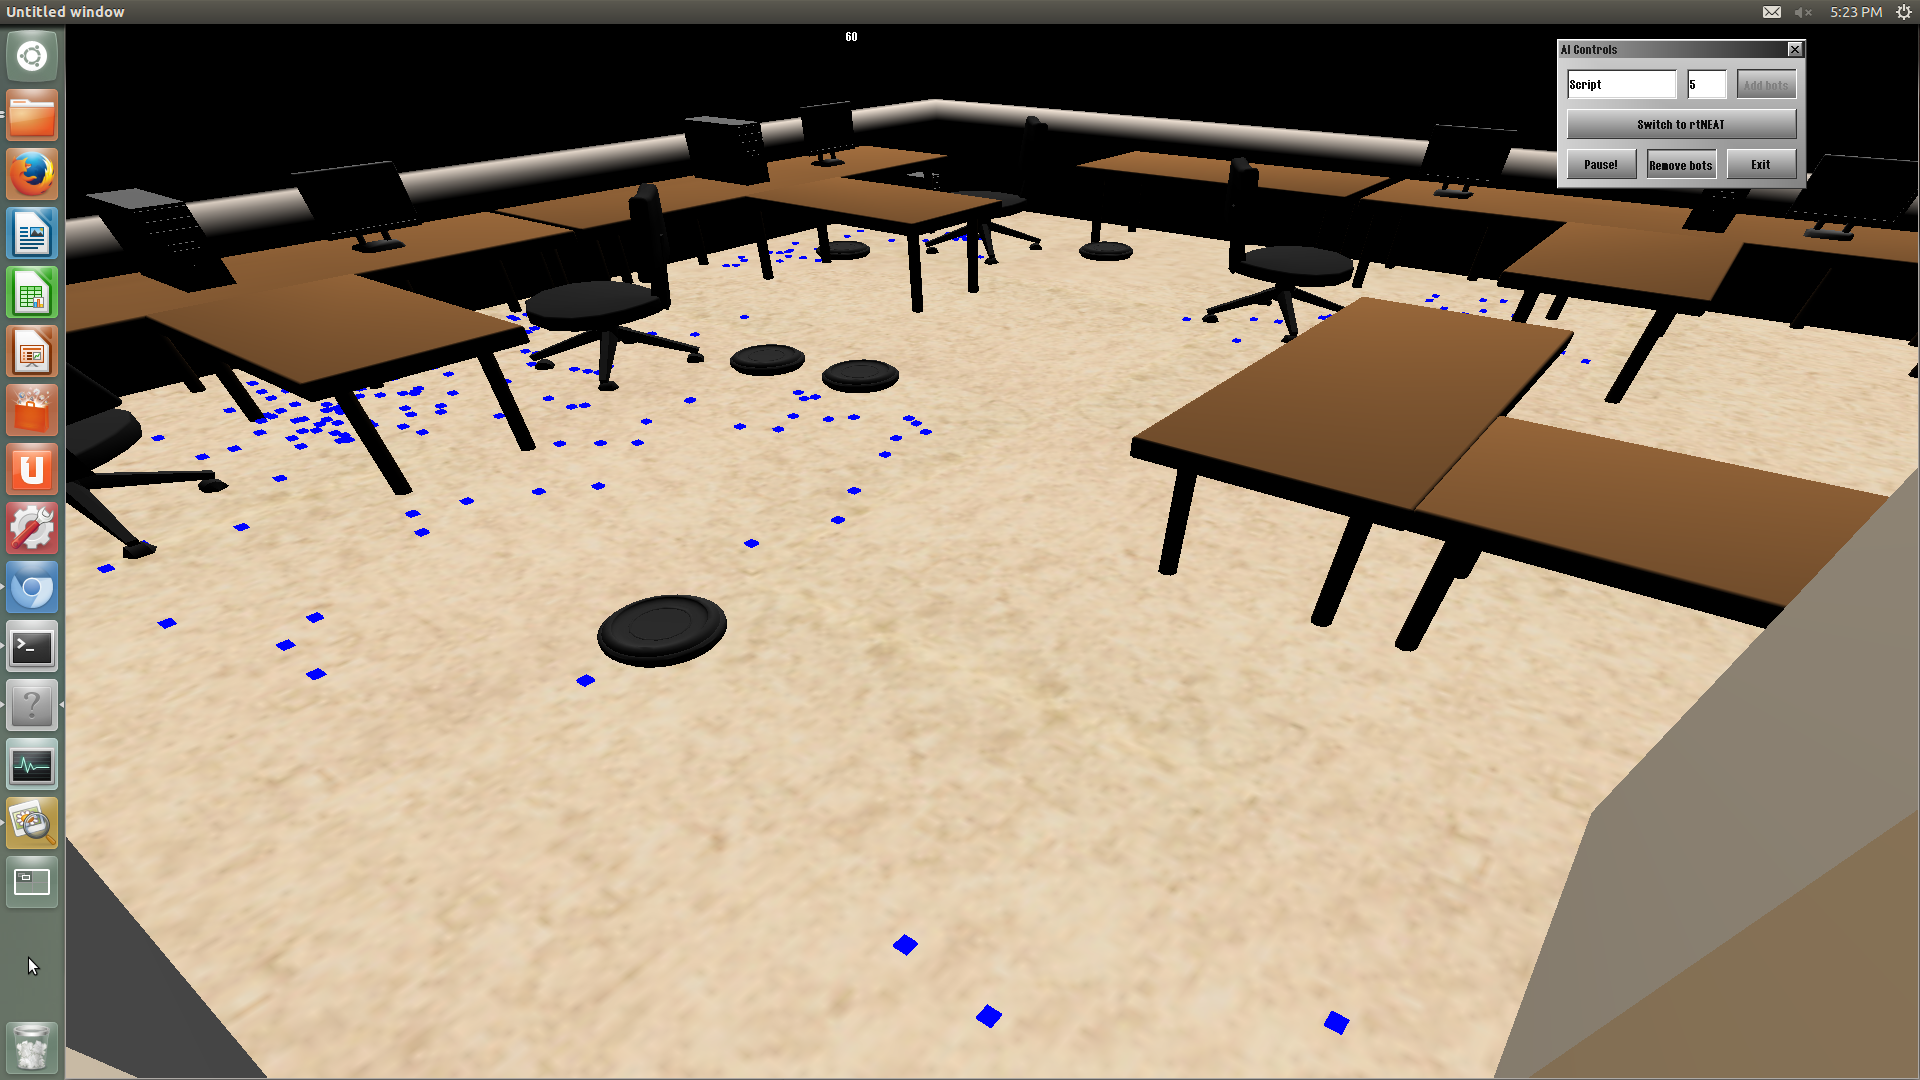
\includegraphics[width=3in,height=2.1in]{./figures/roombas/roomba3.png}
\caption{\textbf{A exempla Roomba robot in the real world.}}
\label{roomba:world}
\end{figure}

\section{Technical Literatures} \label{section:literature}
This section summarizes previous work on multiagent
coordination using reinforcement learning and
neuroevolution techniques.

\subsection{Multiagent Planning as Optimization}
% DCOP
The \textit{Distributed Constraint Optimization Problem} (DCOP), for a long
time, has been a promising approach for modeling distributed reasoning tasks
that arise in multiagent systems, where agents need to coordinate their value
assignments to maximize the sum of the resulting constraint utilities.
Within the DCOP framework, multiagent problems can be solvd efficiently
using fully distributed algorithms which are often based on existing
centralized techniques.  For instances, the OptAPO algorithm
\cite{mailler2004solving} performs partial centralization and serves as an
effective approach to find solutions for the multiagent planning.
In addition, the ADOPT method, introduced in \cite{modi2005adopt}, maintains
distribution of the DCOP and achieves theoretical guarantees on its global
solution.
It also turns out that the degree of allowed centralization has significant impact
on the amount of computation required by an agent \cite{davin2005impact}. 
Other solvers include an utility-propagation method that is amenable to
large-scale multiagent constraint optimization problem
\cite{petcu2005scalable} and an alternating direction method of multipliers
(ADMM) based algorithm \cite{boyd2011distributed}.

% Dyn-DCOP
\textit{Dynamic Distributed Constraint Optimization Problem} (Dynamic DCOP) was
proposed to model dynamically changing multiagent coordination problems.
A dynamic DCOP is a sequence of static DCOPs, each of which partially
different from the DCOP preceding it.
The formulation of Dynamic DCOPs allows us to model problems that
can not be assumed to be static, with particular advantages when the problems
change so frequently that by the time a DCOP solver has found a solution
it is already obsolete. 
Support-Based Distributed Optimization (SBDO) was proposed as a robust method
to solve the Dynamic DCOPs problems \cite{billiau2012sbdo}.

\subsection{Reinforcement Learning Based Coordination}
%######################################################################
%  MDP, DEC-POMDP, and ND-POMDP
\textit{Factored Markov Decision Process} (Factored MDP) is a common model-based
reinforcement learning formulation for cooperative multiagent dynamic systems.
This framework simply views the entire multiagent system as a single, large
MDP, which can be represented in a factored way using a \textit{dynamic Bayesian
    network} (DBN) \cite{guestrin2001multiagent}. 
It implies that the action space of the resulting MDP is the exponential union
of action space of the entire set of agents. 
One effective approach is to employ factored linear value functions as an
approximation to the joint value function, which can be solved simply by a
single linear program \cite{guestrin2001multiagent}. 
A large collection of algorithms are developed based on the factored MDP model. 
These algorithms have a parameterized, structured representation of a policy
or value function, by which agents coordinate both their action selection
activities and their parameter updates and then determine a jointly optimal
action without explicitly considering every possible action in their
exponentially large joint action space \cite{guestrin2002coordinated}. 
However, the factored MDP may not be applicable to the real application due to
its large search space and associated complexity.
To address this problem, the \textit{accelerated gradient method} comes up with
$\mathcal{O}(\epsilon^{-1})$ rate of convergence for solving the distributed
multi-agent planning with Factored MDPs \cite{suegeo2011accgrad}.



%######################################################################
% ND-POMDP
\cite{zhang2011coordinated} This paper presents a
model-free, scalable learning approach that synthesizes
multi-agent reinforcement learning (MARL) and distributed
constraint optimization (DCOP). By exploiting
structured interaction in ND-POMDPs, our approach
distributes the learning of the joint policy and employs
DCOP techniques to coordinate distributed learning to
ensure the global learning performance. Our approach
can learn a globally optimal policy for ND-POMDPs
with a property called groupwise observability. Experimental
results show that, with communication during
learning and execution, our approach significantly outperforms
the nearly-optimal non-communication policies
computed offline.

\cite{nguyen2014decentralized} Existing work typically assumes that the prob-
lem in each time step is decoupled from the problems in other time steps,
which might not hold in some applications. Therefore, in this paper, we make
the following contributions: (i) We introduce a new model, called Markovian
Dynamic DCOPs (MD-DCOPs), where the DCOP in the next time step is a function
of the value assignments in the current time step; (ii) We introduce two
distributed reinforcement learning algo- rithms, the Distributed RVI
Q-learning algorithm and the Dis- tributed R-learning algorithm, that balance
exploration and exploitation to solve MD-DCOPs in an online manner; and (iii)
We empirically evaluate them against an existing multi- arm bandit DCOP
algorithm on dynamic DCOPs.
%######################################################################


\cite{zhang2013coordinating}

\cite{banerjee2012sample}

\cite{kraemer2012informed}

\cite{boukhtouta2011adaptive}
Complex problems involving multiple agents exhibit varying degrees of
cooperation. The levels of cooperation might reflect both differences in
information as well as differences in goals. In this research, we develop a
general mathematical model for distributed, semi-cooperative planning and
suggest a solution strategy which involves decomposing the system into
subproblems, each of which is specified at a certain period in time and
controlled by an agent. The agents communicate marginal values of resources to
each other, possibly with distortion. We design experiments to demonstrate the
benefits of communication between the agents and show that, with
communication, the solution quality approaches that of the ideal situation
where the entire problem is controlled by a single agent.

\cite{sen1994learning}

\subsection{Neuroevolution for Multiagent Coordination}

% Predator prey domain
The \textit{predator-prey problem} has been studied as an application fo neruoevolution. In this problem, several predator agents attempt to capture a fleeing prey. Since the prey is faster than the predators, the agents must learn to cooperate in order to succeed.

% Centralized vs decentralized \cite{yong2001cooperative}
Research by \cite{yong2001cooperative} found that learning is faster in a distributed model where each agent has it's own network, rather than using a single centralized network to coordinate agents' actions.
A more surprising discovery was that communication can actually detract from agents' ability to coordinate. 
Without direct communication, agents were able to coordinate simply by observing each others' changes to the environment. This form of indirect communication is referred to as \textit{stigmergy}, and agents proved to learn faster using stigmergy than direct communication. 

% Communciation vs stigmergy (complex) \cite{rajagopalan2011role}
In a follow up work, \cite{rajagopalan2011role} compared communication and stigmergy in more complicated environments with multiple prey. They discovered that in more complicated environments communicating networks outperform noncomunicating ones. This indicates that while stigmergy is effective when changes to the enviroment are obvious, it becomes increasingly difficult as the enviroment becomes more complicated.

%  Heterogenious vs homogoenous
Work by \cite{bryant2003neuroevolution} shows that multiagent cooperation be achieved with homogeneous networks. Furthermore these networks can be trained such that agents adopt completely distinct strategies despite having identical networks.

Another method for multiagent training is \textit{social learning}. Social learning allows an agent to leverage the knowledge of other networks to enhance the learning process.
In many social learning techniques, agents select a teacher or model, from which they attempt to learn information or behavior \cite{acerbi2006cultural}. This is called the \textit{student-teacher model}, and the success of these methods depends highly on the mechanism by which teachers are selected.

Other social learning approaches do not use the student-teacher method. \textit{Opportunistic Cooperative Learning} (OCL) is a social learning technique designed for multiagent search problems \cite{yang2002ocl}. In OCL, nearby agents can learn from each other, with less successful agents adopting network weights from more successful teammates. 

In another method, called \textit{Egalitarian Social Learning} (ESL), agents also learn from each other without designated teachers \cite{miikkulainen2012multiagent}. In ESL, the population is partitioned into subcultures, with agents free to learn from any member of their subculture. This method helps improve diversity and avoid premature convergence.


\section{The Roomba Environment} \label{section:environment}
To the best of our knowledge, the OpenNERO platform is the best choice for
cheap software simulations. 
The OpenNERO is an open-source platform for artificial intelligence
research and education \cite{karpov2008opennero}. 
The public release of the OpenNERO contains an underdeveloped implementation
of Roomba environment, which supports the communication and coordination of
multiple robots.

\subsection{Structures}
% intro to roomba
The Roomba environment is a virtual office space with crumbs distributed on
the floor.
In this virtual lab, there are four classes of objects: agents, crumbs, walls,
and obstacles. 
Roomba agents, shown as grey cylinders in Fig. \ref{roomba:world}, collect the static crumbs that are depicted as blue cubes.  The
agents automatically pick up all crumbs within a certain radius. 
Walls indicate boundaries of the environment, and other obstacles objects within the virtual environment include tables and chairs. Collision detection for these obstacles can be enabled or disabled in order to vary the complexity of the experiment. For our purposes, only collisions with walls are enabled.

% controller
As shown in the Fig. \ref{roomba:world}, the small window floating on the top right
is the controller that masters the type of scripted AI agents to load in, the
number of agents, and particular commands that impact the progress of the
Roombas simulation (Pause/Resume, Add/Remove Robots, Exit). On each run of the
simulation, only one particular type of AI agents are allowed to be loaded.
Note also that the type of AI agents employed cannot be switched to the other
one during the intermediate process of crumb collection task. 
If one needs to switch to the other type of AI agents, the running agents have
to be removed and then the user is able to effectively load the desired AI agents.

%  movement of agents 

In the Roombas environment, agents have a full $360^\circ$ movement; each action is
denoted as a continuous radius value. All movement is simultaneous, and agent actions are synchronized. 


% placement of pellets 
Three different modes (MANUAL, RANDOM, and CLUSTER) are employed to specify
the placing position of each individual crumb.
In the MANUAL mode, one pellet is deterministically placed at a user-specified
position. 
In the RANDOM mode, the placement of one pellet is totally randomized; the
environment will throw a rejection and repeat the random generation, if an
invalid position is yielded. The last one is the CLUSTER mode, where the
position of pellets are partially randomized. In this mode,
environment samples the position of one pellet from a gaussian distribution
whose centers and spreads at $x$ and $y$ coordinates are specified. 
In this paper, the specifications for the placement of crumbs are generated
from the starting CLUSTER-mode experiment and remained invariant by
employing MANUAL mode in all experiments afterwards.
Note that in any of the three modes, crumb placement does not change when the environment is reset, so agents will train on the same crumb distribution for the lifetime of the environment.

% learning process
The learning process designed in the Roomba environment is as follows. 
The physically dynamic component, consisting of robots and pellets, will be
reset to their initial status once one episode expires. 
Except the spatial positions, all episodic experience and learned knowledge
(i.e. the accumulated Q values from previous episodes) are allowed to preserve
through two adjacent episodes.  
Note that the default configuration for one episode is 100 steps. That is,
for every 100 steps, all agents will be placed back to their birth places no
matter how many pellets they have collected and all crumbs are set at
their specified locations, regardless of whether these crumbs exist at the end
of last episode. 

\begin{figure}[!t]
\centering
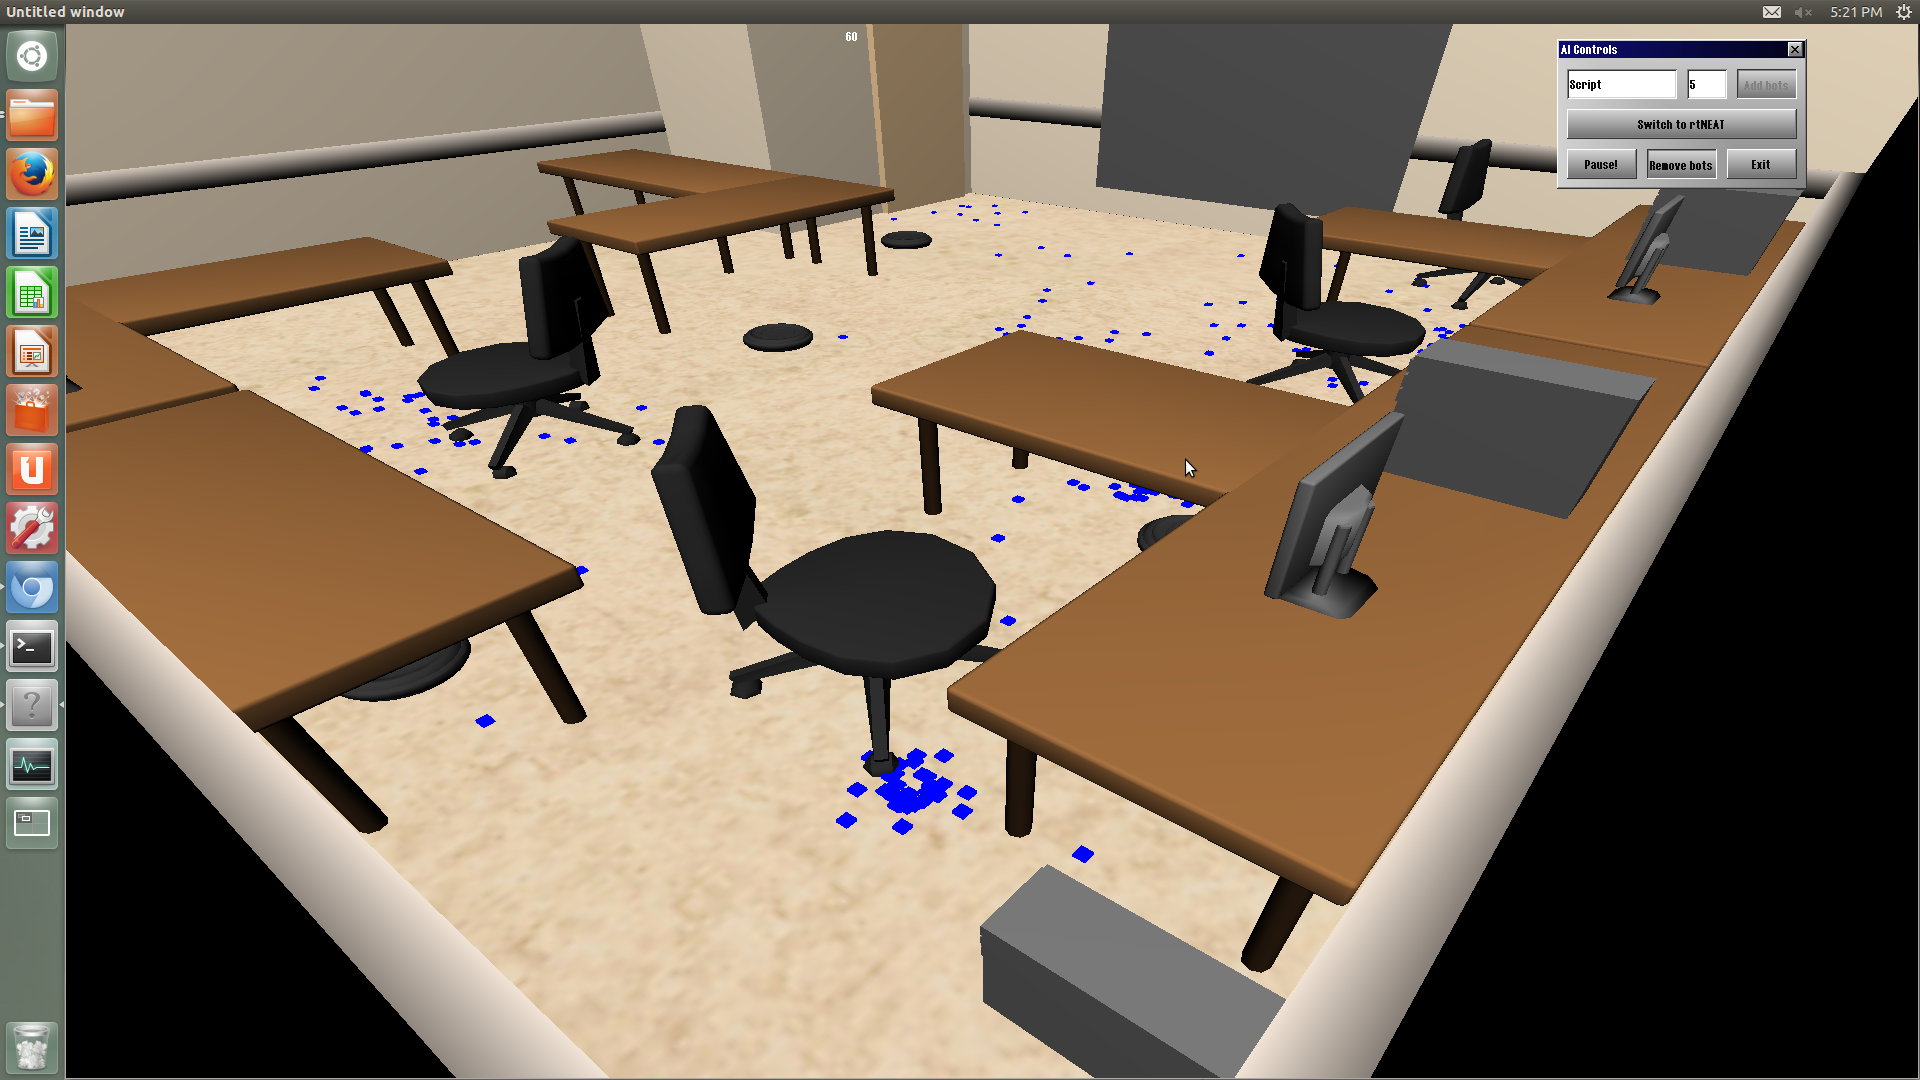
\includegraphics[width=3.2in,height=2.1in]{./figures/roombas/roomba2.png}
\caption{\textbf{Overall Picture of the Roomba Environment}}
\label{roomba:world}
\end{figure}

\subsection{Practical Issues}
% sensors (default setting for greedy agents)
What agents are allowed to perceive from their local views is the practical
issue that matters the most. 
This is important because both of the design of sensors and their
representations have significant impact on the learning outcome of a team. 
The default implementation of Roomba environment allows each agent to sense
all crumbs on the floor about their positions, existing status, and even rewards. 
In this sense, agents are able to perceive limitless information from the
computer lab. 
In addition, the spatial information of other collaborated robots
is available for each individual agent, as well as the user-defined working
status of these teammates (e.g. a history of previous positions and
movements).  Although the Roomba environment provides a large design space for
sensors, it is a practical treatment to start from a small number of simple
sensors. For example, a combination of the bumping status, the position of its
own, and the location of closest crumb suffice for an agent to learn a greedy
strategy, as illustrated in the initial setup experimentation.  

% rewards
The reward design is another big issue for
configuring the Roomba environment. By default, the only reward being set up
for agents is when they successfully collect some pellets on the floor. In
order to facilitate the learning of agents, an penalty for being alive is
supposed to be incorporated to the reward system. That is, agents should
receive some negative rewards, typically a very small quantity, for each step
they move. Similarly, penalties can also be granted to the collisions between
roombas, bumping of agents towards the world boundaries, and repetitive
movements around an area.

\subsection{Expected Multiagent Behaviors}

Workload balance is the foremost coordinative behaviors the
agents should reflect in the Roomba System. This is also known as competition
avoidance. If the workload can be evenly distributed to each agent, in terms of
local perceptions and limited amount of communicative information, the team is
more likely to yield the globally optimal performance.

Another Collision avoidance. 

%\section{Our Approaches}
%This section articulates, in a formal way, our original ideas or design
%priciples to advance the cleaning efficacy of the Roomba environment from the
%multiagent perspective.
%
%\subsection{Tiled Tabular Q-learning} 
%TODO: description of TTQ
%
%\subsection{High-level Reinforcement Learning} 
%TODO: any original idea goes here.
%
%\subsection{Neuroevolution} 

\section{Reinforcement Learning Experiments}
\label{section:rlexpo} 

This section presents our experimental investigation on the thread of reinforcement
learning based agents.

\subsection{Greedy-Random Agents} 
Greedy-random Agents serve as the benchmark for our reinforcement
learning based agents.
Agents with greedy strategy simply approaches to the direction where the
closest pellet to it is there.
The greedy-random agents basically follow such greedy strategy but they make
their final decisions with some probability to make random movements. 
We incorporate such randomness because we need to .

\subsection{Tiled Tabular Q-learning Agents}
The motives to use Tiled Tabular Q-learning include
(i) verifying that we have set up the environment correctly for general
reinforcement learning techniques. 
(ii) illustrating the benchmark (reinforcement learning) intelligence for the
crumb collection problem.

\begin{figure}[!t]
\centering
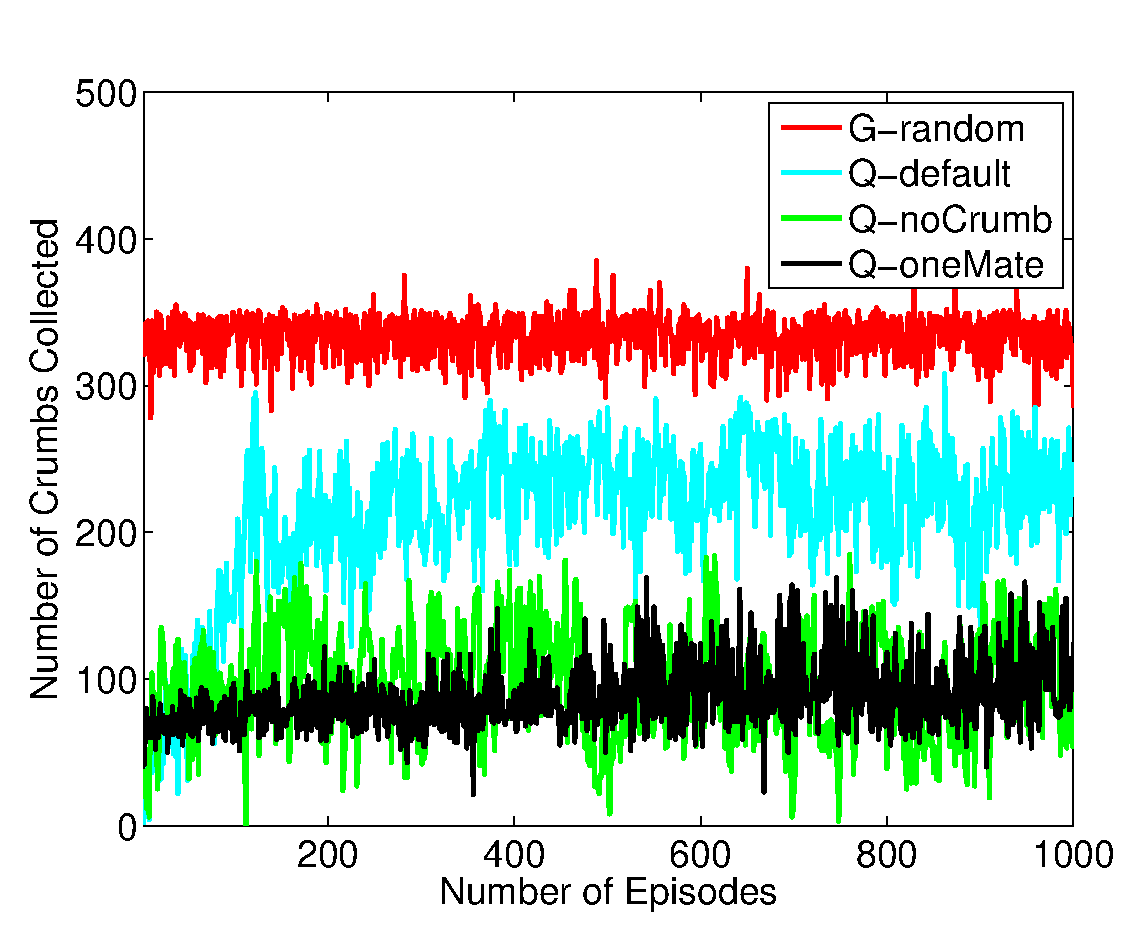
\includegraphics[width=3.0in]{./figures/RL/init_setup1.eps}
\caption{\textbf{Q-learning with various simple sensors.} (i) Red: G-random curve
    represents the greedy agent with $0.1$ probability to make a random
    decision, which serve as the benchmark agents. 
    (ii) (iii) (iv) agents receive various collection of sensors for their
    decision making of each step. Q-noCrumb, Q-default, and Q-oneMate
    represent the learning performances of agents that receive $S_{nc}$,
    $S_{d}$, and $S_{om}$ respectively.
} 
\label{fig:RL_init}
\end{figure}

\begin{figure}[!t]
\centering
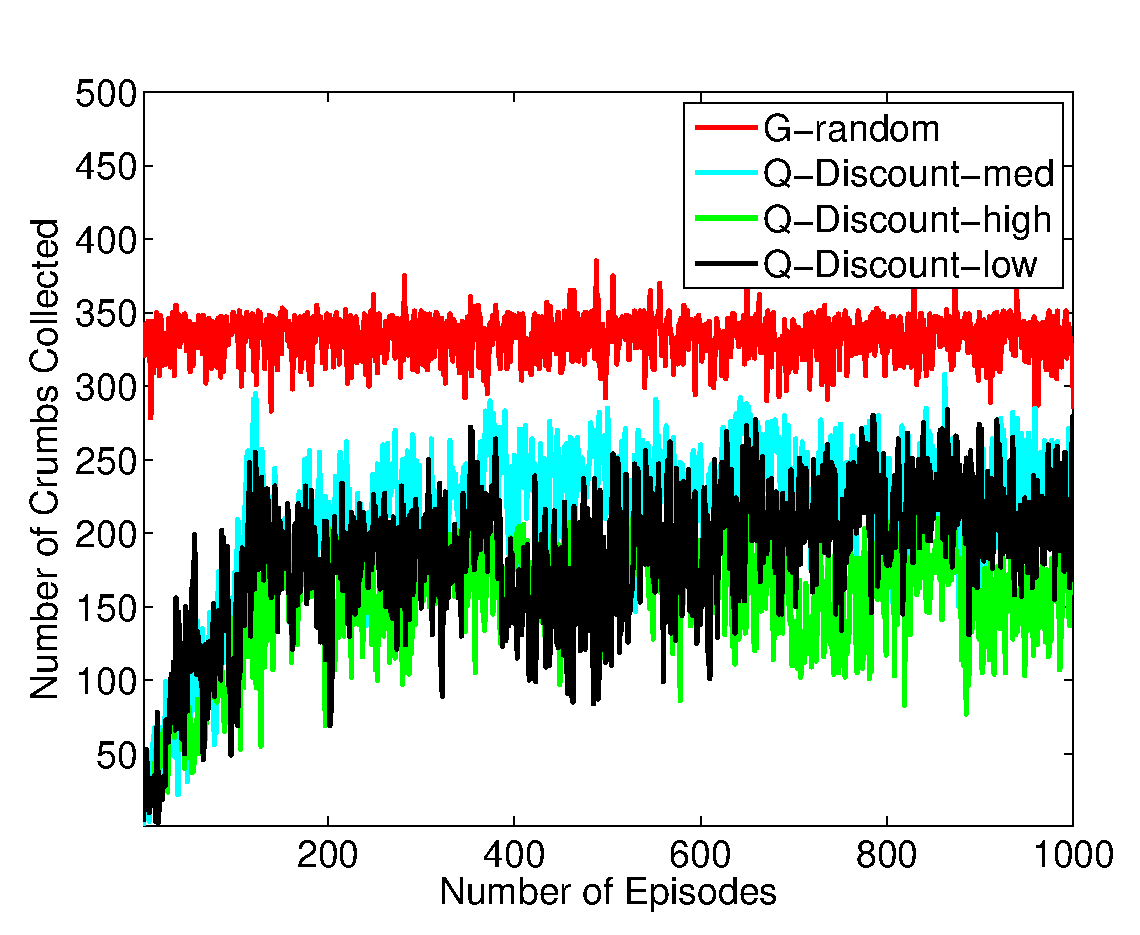
\includegraphics[width=3.0in]{./figures/RL/init_setup2.eps}
\caption{\textbf{Q-learning with various discounting factors.} (i) Red: G-random curve
    represents the greedy agent with $0.1$ probability to make a random
    decision, which serve as the benchmark agents. 
    (ii) (iii) (iv) the tilted tabular Q-learning with discounting factors
    $\gamma = 0.1, 0.5, 0.8$ for Q-Discount-low, Q-Discount-med, and
    Q-Discount-high respectively.}
\label{fig:RL_init2}
\end{figure}

% preliminary results
Before diving into the investigation of multiagent coordination, we take 
preliminary experiments to investigate the impact of various collections of
simple sensors and the effects of various discounting factors on the outcome
of the tiled tabular Q-learning.

TODO: explain some other constans (Number of agents, pellets, )


The sensors designed for the local perspective of each agent are as follows. 
\begin{align}
    S_{nc} = \left( \begin{array}{c}
      self.position.x \\
      self.position.y 
  \end{array} \right)
    S_{d} = \left( \begin{array}{c}
      self.position.x \\
      self.position.y \\
      closestCrumb.x \\
      closestCrumb.y 
  \end{array} \right)
    \nonumber
\end{align}
\begin{align}
        S_{om} = \left( \begin{array}{c}
      self.position.x \\
      self.position.y \\
      closestCrumb.x \\
      closestCrumb.y  \\
      DistToClosestMate.x \\
      DistToClosestMate.y 
  \end{array} \right)
        \nonumber
\end{align}
Note that we discretize all real-value sensors by using the tiling
techniques mentioned in the previous section. 

The learning outcomes derived from these sensors are compared in the
Fig. \ref{fig:RL_init}. 
Observations tell us that the positional information of the closest crumb
tremendously contributes to the quality of agents' learned policies. 
In addition to that, the relative position to the closest collaborated agent
indeed hinder the Q-learning process, such that the communicative agents (black
curve) performs worse than the team that do not monitor collaborators'
positions (light-blue curve) during the observed episodes. One exciting
discovery behind the figure is the narrow performance gap between the team of
tiled tabular Q-learning agents and that of greedy-random agents. It turns out
that the collective works made by naive Q-learning agents even outperform the
team with greedy strategies.



The Fig. \ref{fig:RL_init2} shows the effects that various discounting factors
will bring to the outcome of tilted tabular Q-learning. It turns out that the
best learning outcome came from the discounting factor $\gamma = 0.5$ under
the given setting. On top of that, this chart also indicates the negative
effects of too large or too small discounting factors, by which worse learning
outcome arises. Nevertheless, it can be concluded that the team formed by
tabular Q-learning agents cannot never outperform the team whose members
employ the greedy strategy, regardless of how the discounting factor is set.

% multiagent coordination
\subsection{High-level Reinforcement Learning}
After the preliminary experiments, it is natural to investigate the problem of how
to incorporate effective coordinations for this particular multiagent system.


%#########################################################################

\section{Neuroevolution Experiments}
\label{section:neuro}
%\subsection{Methodology}

In the following experiments, agents were controlled by neural networks
trained using \textit{NeuroEvolution of Augmenting Topologies} (NEAT)
\cite{stanley2002evolving}.
In particular, we evolved these networks with real-time NEAT, which does not use generations -- instead replacing agent's networks without halting the simulation. However, the search space is eventually depleted of crumbs and must be reset. Simulations are therefore divided into \textit{episodes} which last a fixed interval, and  each episode begins by distributing agents and crumbs around the environment. Agents' networks are continually swapped out throughout an episode according to the rtNEAT algorithm.

\subsection{Setup}

\begin{figure}[!t]
\centering
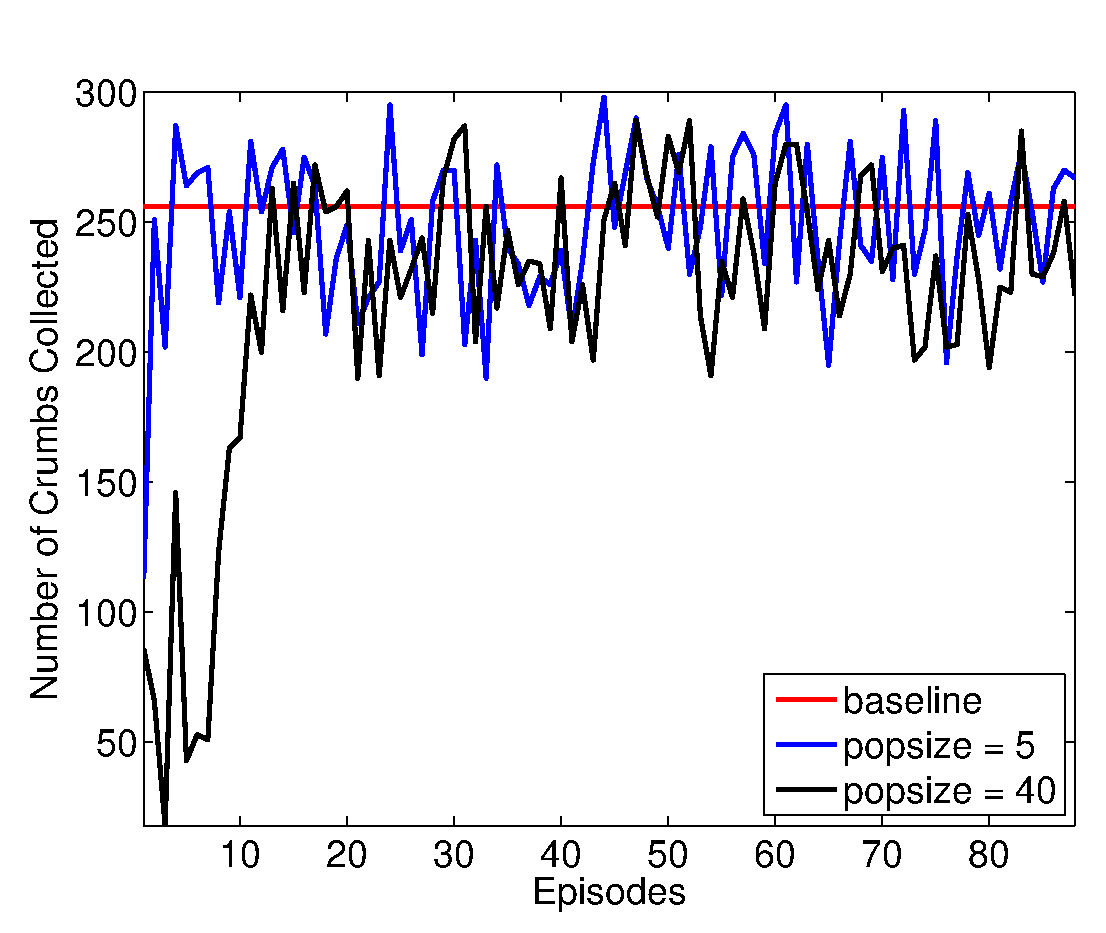
\includegraphics[width=3.0in]{./figures/neroevolution/pop_size.eps}
\caption{\textbf{Effect of population size on neuroevolution.} Demonstrates the effect of choosing different network population sizes in an environment with five agents. Observe that having more networks than agents slows the learning process. Further note that this is using a simple one input / one output network; with a more complicated network, the large population shows only marginal results even after 1,000 episodes.}
\label{neroevolution:pop_size}
\end{figure}

Experiments using the original configuration of the Roomba module yielded poor results. Agents' performance did not increase over time.  Even after hundred of episodes, no evidence of learning occurred. This section discusses the steps necessary to enable even basic training of the Roomba agent. These results serve as a yardstick for later experiments on multiagent coordination.

In order to facilitate learning, a larger population size is necessary. 
However, anything more than a handful of Roombas quickly picks up all of the crumbs, even when moving in random directions. This creates difficulties when attempting to compare the results of different experiments.
One solution is to have a large population of networks of which only a small number are used by agents at a given time. Fig.\ref{neroevolution:pop_size} shows that this approach considerably slows the learning process. For complicated networks, this approach quickly becomes unfeasible.

One can avoid this issue by scaling the number of agents to match the network population size. These modification present an issue, however, as the Roombas often manage to collect all of the available crumbs before time expires. In order to prevent this, our methodology has been to reduce agents' size and speed such that they are unable to collect every crumb before an episode ends. Additionally, the total time taken to collect all crumbs was compared as a secondary performance metric.


\subsection{Fitness}
Originally, an agent's fitness was based purely on collecting crumbs. Various other mechanisms were considered, including the ability to avoid obstacles and other agents. Experimental evidence showed the best results came from moderately penalizing collisions while heavily rewarding crumb collection. The fitness function for these experiments is:


\[ fitness = \phi * n_{crumbs} - \psi * n_{collisions}\]

Where $n_{curmbs}$ is the number of crumbs collected and $n_{collisions}$ the number of wall collisions over the course of an episode. 
 
Performance generally improved with increases to either $\phi$ or $psi$.
Interestingly, combining high values for both $\phi$ and $\psi$ resulted in worse performance than increasing either value individually, suggesting that the two behaviors interfere with each other in some way. 
Experimentally derived results show $\phi = 1, \psi = 0.05$ as good choices, which moderately incentively collision avoidance while primarily focusing on crumb collection. 

% % % unnecessary????
% \begin{figure}[!t]
%\centering
%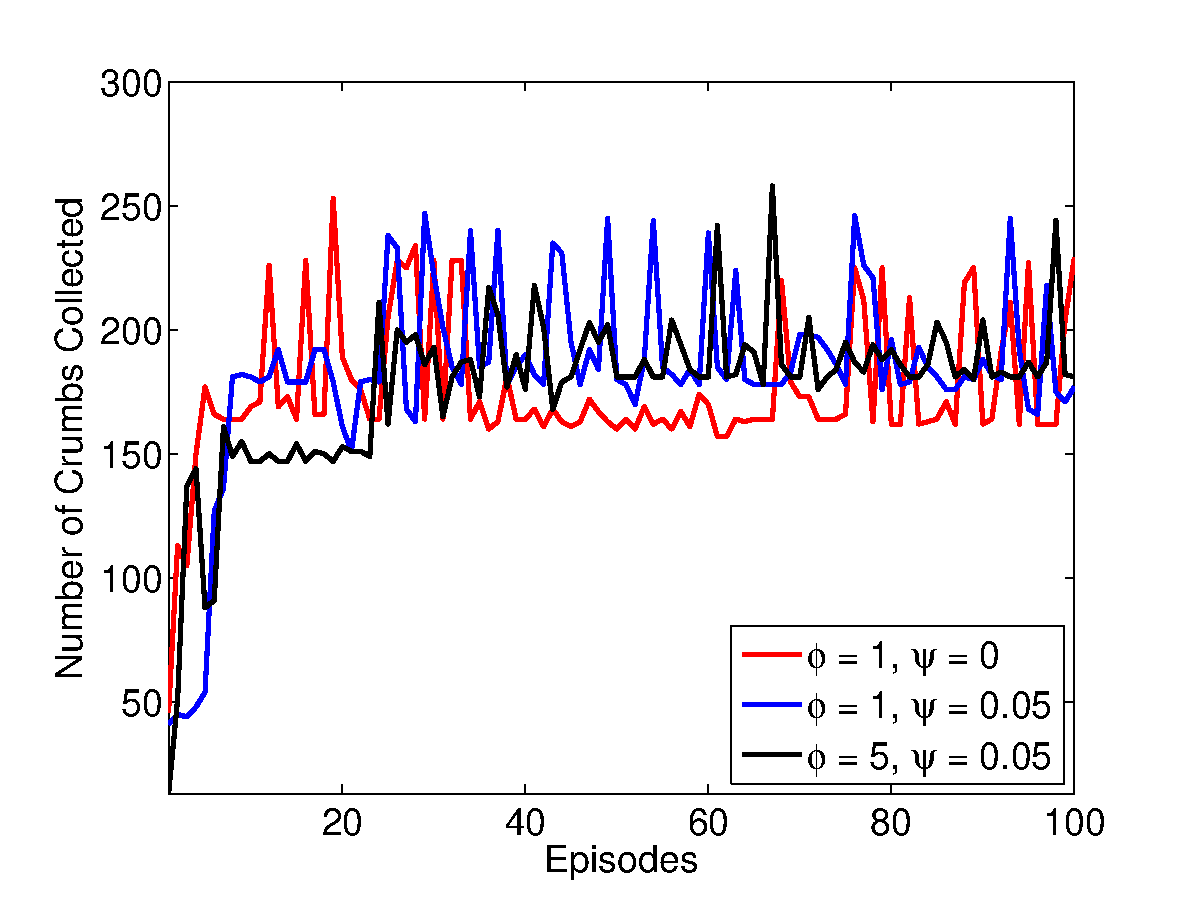
\includegraphics[width=3.3in]{./figures/neroevolution/reward.eps}
%\caption{Comparison of fitness functions}
% \label{neroevolution:fitness}
%\end{figure}


\subsection{Neuroevolution Baseline}

In all of our experiments, we compare the results of neuroevolution against hardcoded search behavior as a baseline. This baseline consists of a simple greedy algorithm -- each agent always moves directly towards the nearest crumb. Obviously, this is not an optimal algorithm, and we hope to show that neroevolution can produce a superior result. In particular, the greedy algorithm's agents do not coordinate their efforts. We hope that our evolved agents will learn to better cooperate in order to perform a better search of the target space.

%Single sensor
For a starting point, the simplest possible network is trained to match the behavior and performance of the greedy algorithm. A single sensor detects the nearest crumb. The network receives the angular direction to that crumb as input, and outputs the angular direction the roomba should turn to face. In order to emulate the behavior of the greedy algorithm, the network needs only to map the input directly to the output. Unsurprisingly, the network learns this behavior very quickly.

%2 sensor better than script
In order to improve over the greedy algorithm, it suffices to add just one more sensor. This sensor detects the distance to the nearest crumb. Equipped with both an angle and distance to the crumb, the network now learns behavior superior to the greedy algorithm.

This result is both logical and significant. It demonstrates that agents learn to leverage the additional information of how far away a crumb is. An agent is more likely to capture nearby crumbs, improving its fitness. When the crumb is further away, however, it is more likely that another agent will reach that crumb first. Thus, the agent has better odds by moving to another area. 
One might wonder if agents could benefit from additional sensors detecting furhter away crumbs. In practice, however, there was improvement from simply adding sensors that pointed to further crumbs.

\begin{figure}[t]
\centering
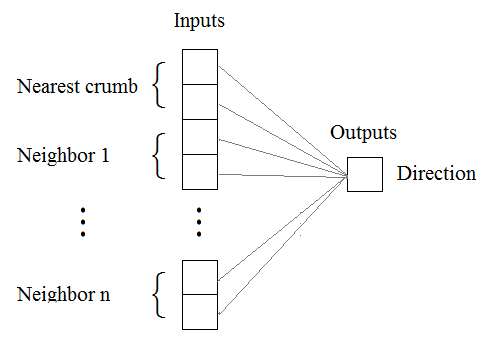
\includegraphics[width=3.0in]{./figures/neroevolution/comm_network.png}
\caption{\textbf{Communicating Roomba network.} Initial network to be evolved with rtNEAT. Sensors detect the polar offsets (angle and magnitude) of the $n$ nearest neighboring agents, as well as the nearest crumb. Output represents the (angular) direction in which the agent should move.}
\label{neroevolution:communication}
\end{figure}

\begin{figure}[t]
\centering
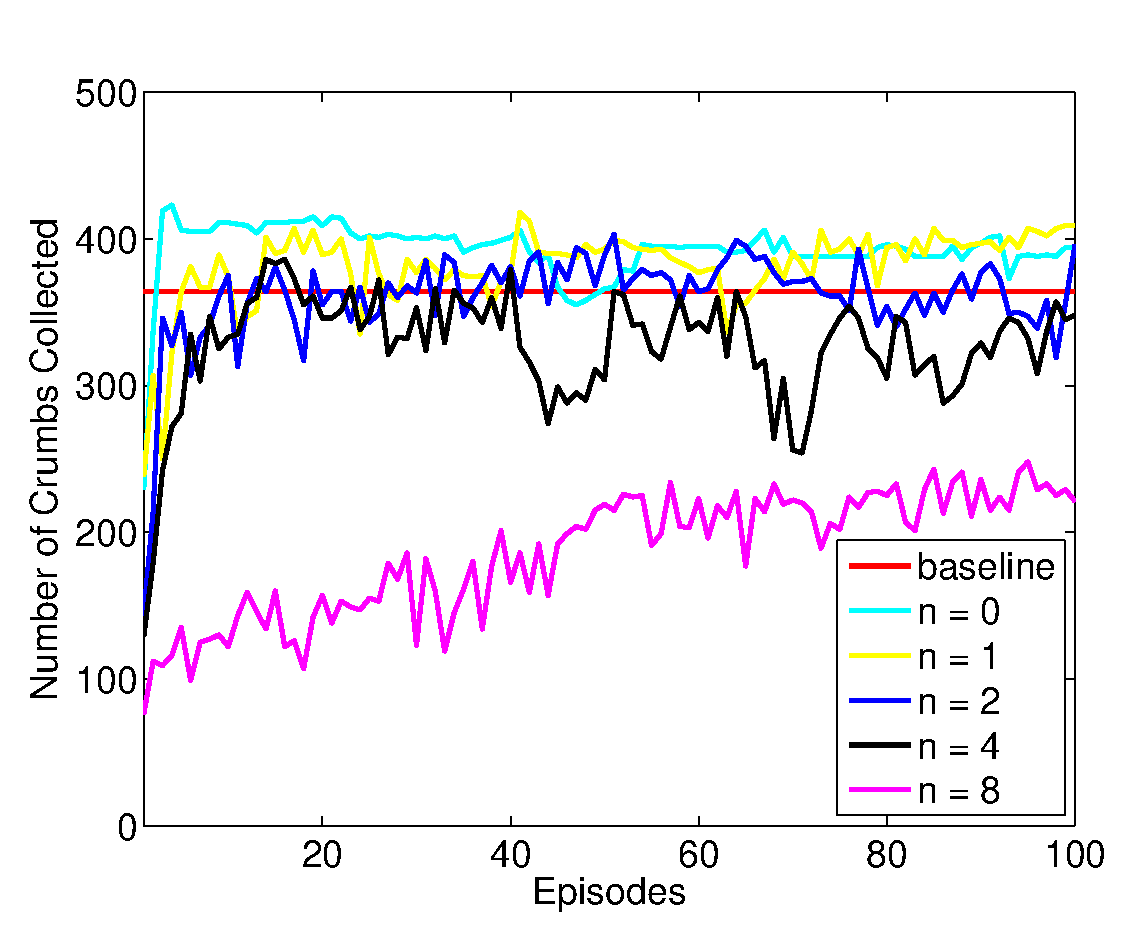
\includegraphics[width=3.0in]{./figures/neroevolution/comm_result.eps}
\caption{\textbf{Communicating Roomba results.} Comparison of non-communicating agents ($n=0$) with communicating ones. The more neighbors an agent communicates with, the slower it learns. Furthermore, none of the communicating agents exceed the performance of non-communicating ones, with more communication in fact resulting in worse performance. }
\label{neroevolution:communication_results}
\end{figure}

\subsection{Communication}

%Communication

We have establishes that training with rtNEAT can outperform the hardcoded greedy algorithm. However, agents are still entirely independent, not directly sharing information. An argument can be made that they are indirectly coordinating through the position of crumbs in the environment, but one wonders if better results can be achieved through direct communication.

The network design, shown in Fig. \ref{neroevolution:communication}, is straightforward. Inputs consist of the offset of the nearest crumb as well as that the nearest $n$ agents. Offsets are polar, consisting of an angular direction and a scalar magnitude. As before, the single output represents the angular direction the agent will turn to face. 
This section compares experimental results for different choices $n$, where $n=0$ represents no communication, and each increment adds another neighbor to each agent's awareness.

As seen in Fig. \ref{neroevolution:communication_results}, the more neighbors the agent communicates with, the longer it takes to learn.  Fig. \ref{neroevolution:communication_results} shows that the $n=1$ neighbor network catches up with the $n=0$ network after about 20 episodes. The other networks, however do not reach this level even after several hundred episodes of training. Note that while the networks appear to cap out at 400 crumbs per episode, there are approximately 30-50 crumbs uncollected at this point. So while there is still room for improvement over the $n=0$ network, none of the communicating networks achieve better results. In fact the networks with higher $n$-values do \textit{worse} than the non-communicating network, plateauing at significantly lower crumb counts.

%Shared fitness
Previous research by \cite{rajagopalan2011role} has showed that sharing fitness functions between agents can improve multi-agent learning. 
To explore this, we use a modification of the Roomba environment to share fitness amongst agents. Instead of being rewarded only when picking up a crumb, agents share the reward from their teammates success. 

Fig. \ref{neroevolution:shared_fitness} show the results for a non-communicating network ($n=0$) and a network which observes one neighbor ($n=1$). In both cases, the shared fitness networks perform abysmally, showing no learning whatsoever.

\begin{figure}[t]
\centering
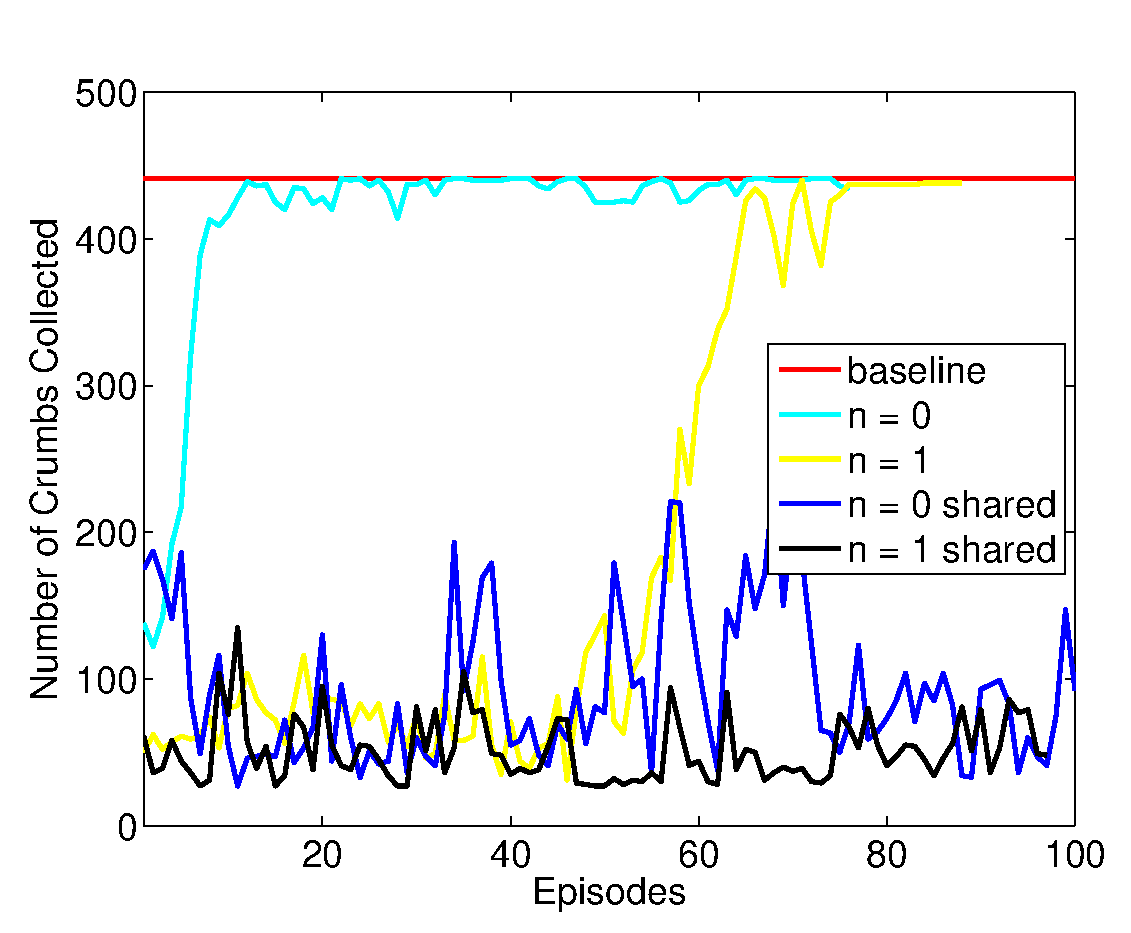
\includegraphics[width=3.0in]{./figures/neroevolution/shared_result.eps}
\caption{\textbf{Comparison of individual vs shared fitness.}}
\label{neroevolution:shared_fitness}
\end{figure}

\subsection{Evolved Communication}

Counterintuitive, these experiments have shown that communication is in fact detrimental to the learning process.
However, conveying the location of fellow agents is a very simple form of communication. It is possible that with different signals and messages, the agents could learn to use communication to their advantage.

One way to test this is to have the network evolve its own communication (Fig. \ref{neroevolution:evolved_comunication}). Each network is given an additional output -- a signal to broadcast. As input, the agent senses the direction and strength of signal being broadcast from it's $n$ nearest neighbors. 

In order for communication to be valuable, agents must have information to share. 
Each agent is equipped with a sensor which detects how many crumbs are within a small radius. A radius of 1/8 of the length of the environment was chosen through experimentation -- larger radii rendered the sensor useless.

\begin{figure}[t]
\centering
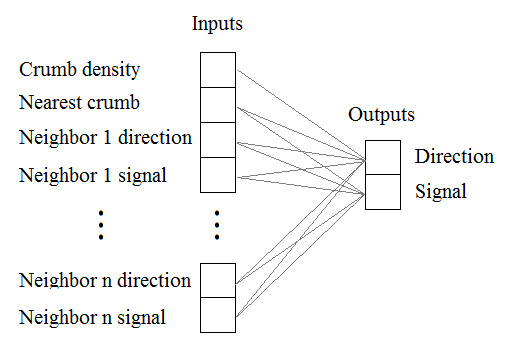
\includegraphics[width=3.0in]{./figures/neroevolution/emerg_comm_network.png}
\caption{\textbf{Communicating Roomba network with evolved signals.} The addition of a broadcast signal gives agents a more expressive means of communication. This network receives the direction of and signal being broadcast by each of the $n$ nearest neighboring agents. It also has stronger information about its local environment, receiving both the density of nearby crumbs as well the angle to the nearest crumb.  }
\label{neroevolution:evolved_comunication}
\end{figure}

The goal is for agents to learn to communicate their short range observations to each other in order to improve their overall performance.
Unfortunately, results were little better than with the simple communicating network (Fig. \ref{neroevolution:evolved_comunication_results}). 
Again, the more neighbors communicated with, the longer it took a network to learn. Ultimately, the higher $n$-value networks did reach the same performance as the 0-neighbor network, but not until over 500 episodes. Whereas the 0-neighbor network peeked within 10 episodes, and the 1-neighbor in about 25. At no point did any of the communicating networks consistently outperform the $n=0$ network. Nether did this communication with evolved signal perform any better than the simple communication of neighbors' location. 

\begin{figure}[t]
\centering
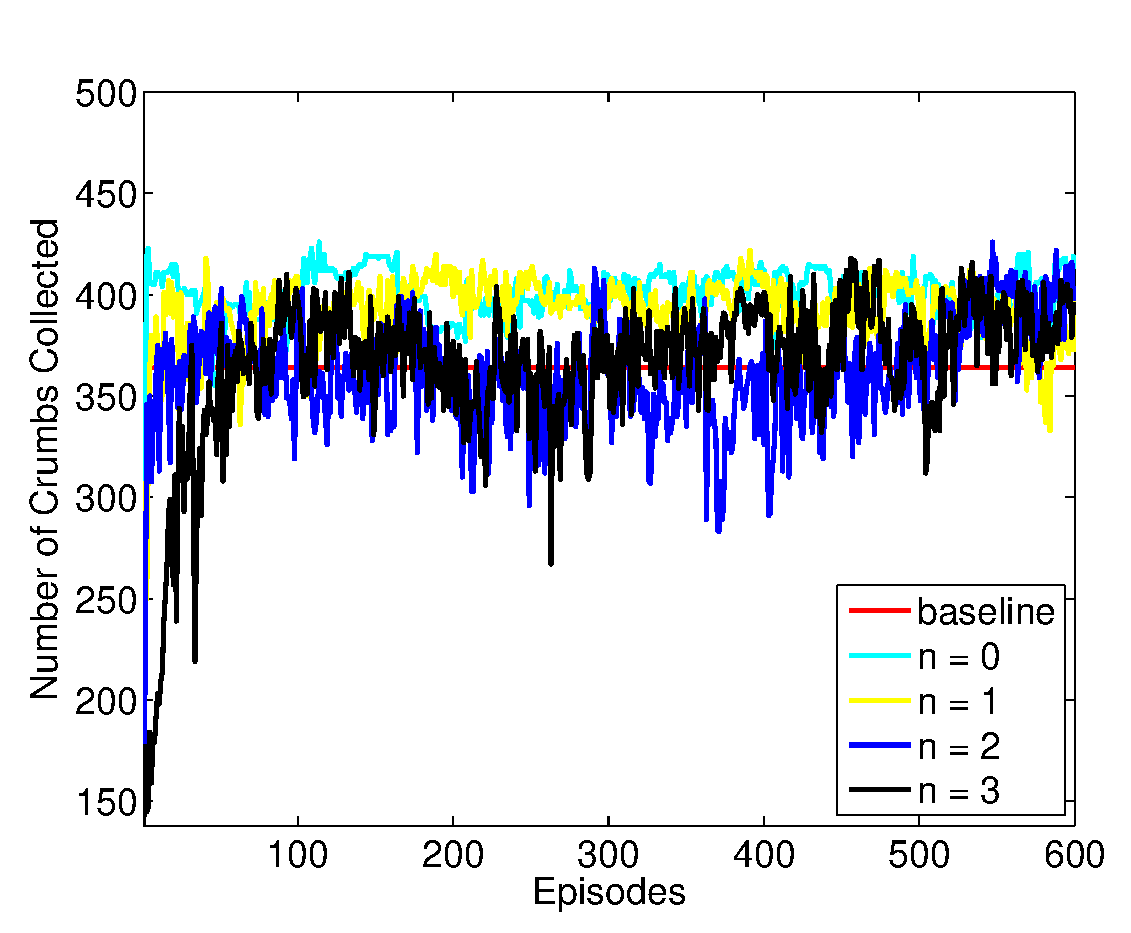
\includegraphics[width=3.0in]{./figures/neroevolution/emerg.eps}
\caption{\textbf{Comparison of evolved communication.} Over a long timespan, the higher $n$-value networks eventually reach, but do not exceed the performance of the non-communicating ($n=0$) network. For any $n>1$, this takes several hundred episodes. }
\label{neroevolution:evolved_comunication_results}
\end{figure}


%neroevolution conclusion
%Say something about how, surprisingly, communication can actually hurt network performance.

\section{Conclusions} \label{conclusion}
The conclusion goes here. In this paper, we investigate.

Promising future Works go here.

% trigger a \newpage just before the given reference
% number - used to balance the columns on the last page
% adjust value as needed - may need to be readjusted if
% the document is modified later
%\IEEEtriggeratref{8}
% The "triggered" command can be changed if desired:
%\IEEEtriggercmd{\enlargethispage{-5in}}

% references section

% can use a bibliography generated by BibTeX as a .bbl file
% BibTeX documentation can be easily obtained at:
% http://www.ctan.org/tex-archive/biblio/bibtex/contrib/doc/
% The IEEEtran BibTeX style support page is at:
% http://www.michaelshell.org/tex/ieeetran/bibtex/

\bibliographystyle{IEEEtran}
\bibliography{report}

% <OR> manually copy in the resultant .bbl file
% set second argument of \begin to the number of references
% (used to reserve space for the reference number labels box)

%\begin{thebibliography}{1}
%\bibitem{IEEEhowto:kopka}
%H.~Kopka and P.~W. Daly, \emph{A Guide to \LaTeX}, 3rd~ed.\hskip 1em plus
%  0.5em minus 0.4em\relax Harlow, England: Addison-Wesley, 1999.
%\end{thebibliography}




% that's all folks
\end{document}
